\section{Linear Regression}

\begin{frame}{Pearson Correlation Coefficient}

    The Pearson correlation coefficient for a population:
    \begin{equation}
    \rho = \frac{cov(X, Y)}{\sigma_X \sigma_Y}
    \end{equation}
    
    The Pearson correlation coefficient for a sample:
    \begin{equation}
    r = \frac{\sum_{i=1}^{n}(x_i - \bar{x})(y_i - \bar{y})}{\sqrt{\sum_{i=1}^{n}(x_i - \bar{x})^2}\sqrt{\sum_{i=1}^{n}(y_i - \bar{y})^2}}
    \end{equation}
    
    $\rho$ and $r$ have values between +1 and -1, where 1 is total positive linear correlation, 0 is no linear correlation, and -1 is total negative linear correlation.
    
\end{frame}

\begin{frame}{Pearson Correlation Coefficient}
    \begin{figure}
    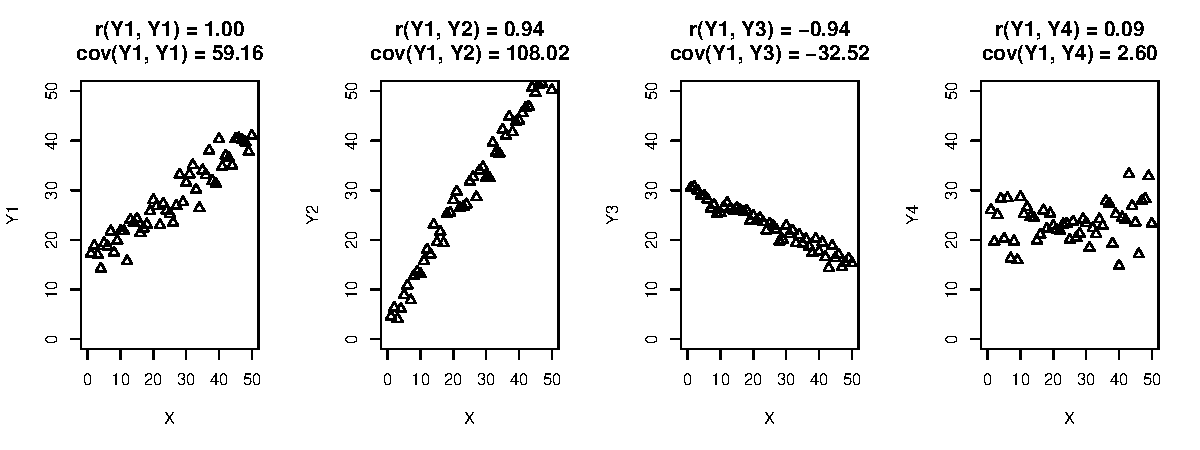
\includegraphics[width=\linewidth]{R/plots/pearson.pdf}
    Pearson correlation coefficient vs. covariance
    \end{figure}

    {\tiny R commands: \texttt{cor}, \texttt{cov}}
\end{frame}

\begin{frame}{Linear Regression}
    
    \textbf{Linear regression} is a simple approach for predicting quantitative responses using linear models.
    
    E.g. linear regression can be used to answer the following questions:
    {\small
    \begin{enumerate}
        \item Is there a relationship between advertising budget and sales?
        \item How strong is the relationship between advertising budget and sales?
        \item Which media (TV, radio, newspapers) contribute to sales?
        \item How accurately can we estimate the effect of each medium on sales?
        \item How accurately can we predict future sales?
    \end{enumerate}}
    
\end{frame}

\begin{frame}{Simple Linear Regression}
    
    For the prediction of a single quantitative response $Y$ based on a single predictor variable $X$, we can assume a linear relationship between them:
    \begin{equation}
    Y \approx \beta_0 + \beta_1 X
    \end{equation}  
    The are two \emph{coefficients} (or parameters) in this model:\\
    $\beta_0$ -- intercept, $\beta_1$ -- slope. The \emph{true coefficients are unknown}, but we can estimate them.

    \begin{figure}
        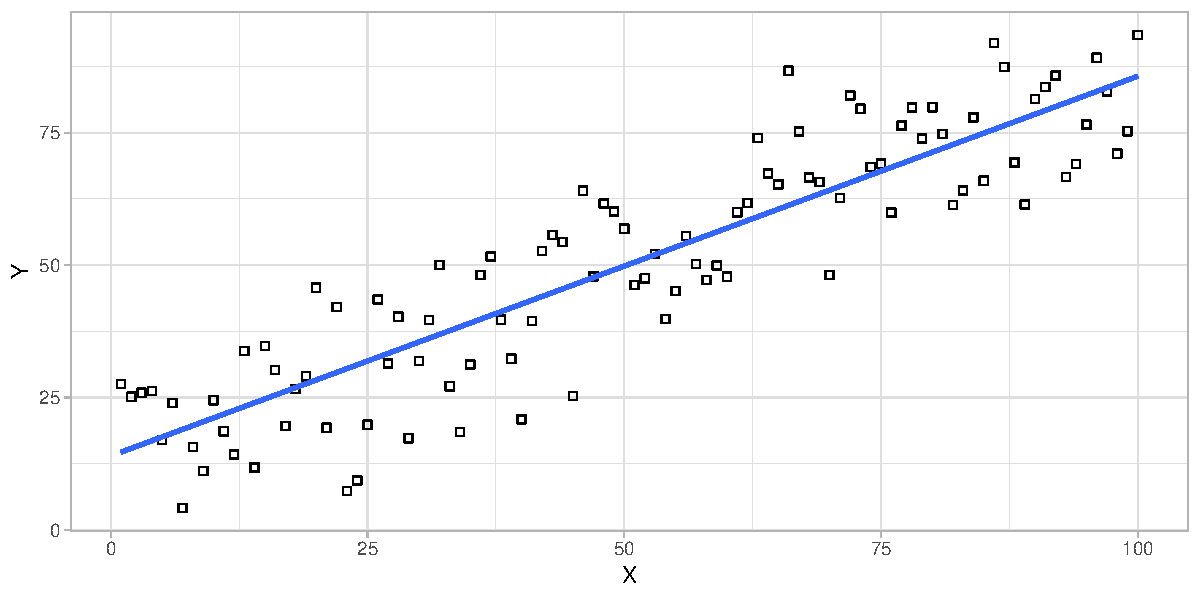
\includegraphics[width=0.7\linewidth]{R/plots/linear_regression}
    \end{figure}

\end{frame}

\begin{frame}{Estimating the Coefficients: Ordinary Least Squares}

    Let $\hat{y}_i = \hat{\beta}_0 + \hat{\beta}_1 x_i$ be the prediction for $Y$ based on the $i$th value of $X$. Then the $i$th residual is given by:
    \begin{equation*}
    e_i = y_i - \hat{y}_i,
    \end{equation*}
    and the \emph{residual sum of squares} (RSS) is as follows:
    \begin{align*}
    \text{RSS} = S(\hat{\beta}_0, \hat{\beta}_1) &= e_1^2 + e_2^2 + ... + e_n^2 =\\
                &= (y_1 - \hat{\beta}_0 - \hat{\beta}_1 x_1)^2 + ... + (y_n - \hat{\beta}_0 - \hat{\beta}_1 x_n)^2 =\\
                &= \sum_{i=1}^{n} (y_i - \hat{\beta}_0 - \hat{\beta}_1 x_i)^2
    \end{align*}
    In order to get the coefficients estimates $\hat{\beta}_0$ and $\hat{\beta}_1$ we need to minimize $S(\hat{\beta}_0, \hat{\beta}_1)$.

\end{frame}

\begin{frame}{Estimating the Coefficients: Ordinary Least Squares}
    \label{page:lm-coefficients}
    
    We know that $S(\hat{\beta}_0, \hat{\beta}_1)$ is at the minimum when:
    \begin{equation*}
    \frac{\partial S}{\partial \hat{\beta}_0} = 0,\quad \frac{\partial S}{\partial \hat{\beta}_1} = 0
    \end{equation*}

    We need to solve the following system of equations:    
    \begin{equation*}
    \left\{
    \begin{array}{ll}        
    \frac{\partial}{\partial \hat{\beta}_1} \sum_{i=1}^{n} (y_i - \hat{\beta}_0 - \hat{\beta}_1 x_i)^2 = 0\\
    \frac{\partial}{\partial \hat{\beta}_0} \sum_{i=1}^{n} (y_i - \hat{\beta}_0 - \hat{\beta}_1 x_i)^2 = 0
    \end{array}
    \right.
    \end{equation*}
    
    After some calculus we get the following solution:
    \begin{equation}\label{eq:lm-coefficients}
    \left\{
    \begin{array}{ll}        
    \hat{\beta}_1 = \frac{\sum_{i=1}^{n} (x_i - \bar{x})(y_i - \bar{y})}{\sum_{i=1}^{n} (x_i - \bar{x})^2} = \frac{\text{Cov}(x,y)}{\text{Var}(x)}\\
    \hat{\beta}_0 = \bar{y} - \hat{\beta}_1 \bar{x}
    \end{array}
    \right.
    \end{equation}
    
\end{frame}

\begin{frame}{Estimating the Coefficients: Ordinary Least Squares}
    
    Solving for $\beta_0$:
    \begin{align*}
    &\frac{\partial}{\partial \beta_0} \sum_{i=1}^{n} \left(
        y_i^2 - 2 y_i \beta_0 - 2 y_i x_i \beta_1 + \beta_0^2 + 2 x_i \beta_0 \beta_1 + x_i^2 \beta_1^2
    \right) = 0\\
    &\sum_{i=1}^{n} (-2y_i + 2 \beta_0 + 2\beta_1 x_i) = 0\\
    &\sum_{i=1}^{n} \beta_0 = \sum_{i=1}^{n} (y_i - \beta_1 x_i)\\
    &\beta_0 = \frac{\sum_{i=1}^{n} y_i}{n} - \beta_1 \frac{\sum_{i=1}^{n} x_i}{n}\\
    &\beta_0 = \bar{y} - \beta_1 \bar{x}
    \end{align*}    

\end{frame}

\begin{frame}{Estimating the Coefficients: Ordinary Least Squares}

    Solving for $\beta_1$:
    \begin{align*}
    \frac{\partial}{\partial \beta_0} \sum_{i=1}^{n} &\left(
        y_i^2 - 2 y_i \beta_0 - 2 y_i x_i \beta_1 + \beta_0^2 + 2 x_i \beta_0 \beta_1 + x_i^2 \beta_1^2
    \right) = 0
    \end{align*}

    After substituting $\beta_0$ we get:
    \begin{align*}
    \frac{\partial}{\partial \beta_0} \sum_{i=1}^{n} &\left(
        y_i^2 - 2y_i \bar{y} + 2y_i \bar{x} \beta_1 - 2y_i x_i \beta_1 + \bar{y}^2 -2\bar{x}\bar{y}\beta_1 + \bar{x}^2\beta_1^2 + \right.\\
        &\left. + 2x_i \bar{y}\beta_1 - 2x_i\bar{x}\beta_1^2 + x_i^2 \beta_1^2
    \right) = 0\\
    \beta_1 \sum_{i=1}^{n} &\left( \bar{x}^2 - 2\bar{x}x_i + x_i^2 \right) = \sum_{i=1}^{n} \left( y_i x_i + \bar{x}\bar{y} + y_i \bar{x} - x_i \bar{y} \right)\\
    \beta_1 = &\frac{\sum_{i=1}^{n} (x_i - \bar{x})(y_i - \bar{y})}{\sum_{i=1}^{n} (x_i - \bar{x})^2} = \frac{\text{Cov}(x,y)}{\text{Var}(x)}
    \end{align*}    

\end{frame}

\begin{frame}{Linear Regression Example}
    \begin{example}
        \medskip
        Generate a sample $X$ from the normal distribution $\mathcal{N}(\mu=10, \sigma=2)$. Generate a sample $Y = 0.5X +  \epsilon$, where $\epsilon \sim \mathcal{N}(\mu=0, \sigma=1)$. 
        
        Calculate the linear regression coefficients (Eq. \ref{eq:lm-coefficients}, slide \ref{page:lm-coefficients}) and make a plot visualizing the correlation.
    \end{example}
\end{frame}

\begin{frame}{Assessing the Accuracy of the Coefficient Estimates}

    All these lines were generated from the same model, using five different samples:
    \begin{equation*}
    Y = 15 + 0.5 X + \epsilon,\quad  \epsilon \sim \mathcal{N}(\mu = 0, \sigma = 10)
    \end{equation*}
    \begin{figure}
        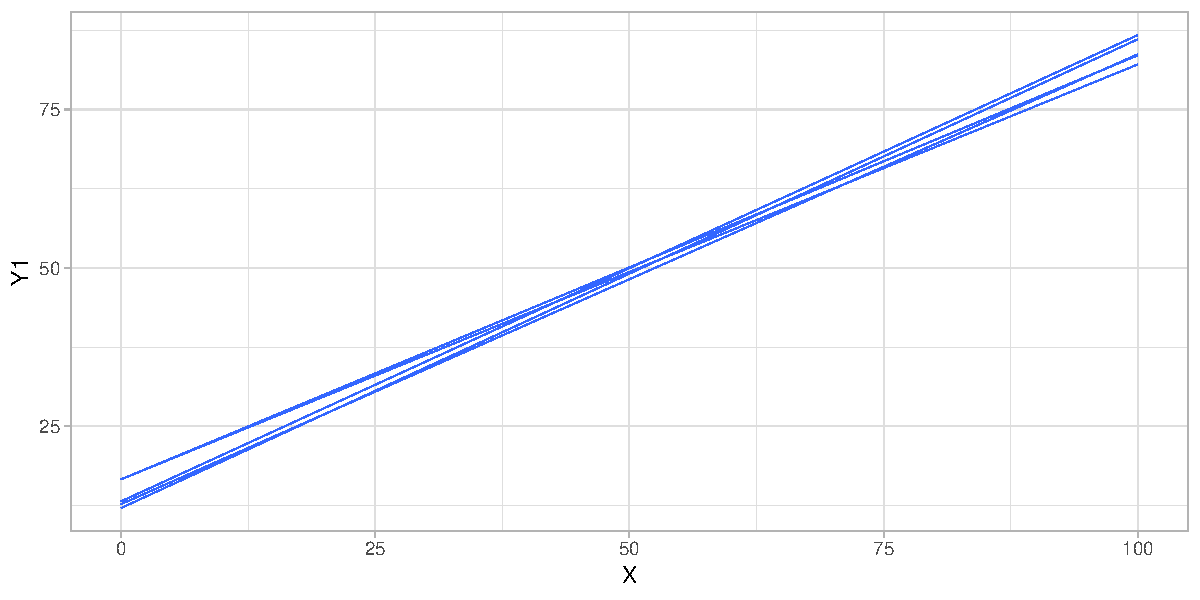
\includegraphics[width=0.8\linewidth]{R/plots/linear_regression_acc}
    \end{figure}
    Which line describes best the real population?

\end{frame}

\begin{frame}{Assessing the Accuracy of the Coefficient Estimates}

    $\hat{\beta}_0$ and $\hat{\beta}_1$ are only estimates of the real coefficients $\beta_0$ and $\beta_1$:
    \begin{equation*}
    Y = \beta_0 + \beta_1 X + \epsilon
    \end{equation*}
    
    If we assume that $\epsilon$ is a zero-mean random error with the standard deviation $\sigma_\epsilon$, then we can derive formulas for the standard errors of $\hat{\beta}_0$, $\hat{\beta}_1$:
    \begin{align}
    SE_{\hat{\beta}_0} &= \sqrt{\sigma_{\epsilon}^2 \left[
            \frac{1}{n} + \frac{\bar{x}^2}{\sum_{i=1}^{n} (x_i - \bar{x}^2)}        
        \right]}\\
    SE_{\hat{\beta}_1} &= \sqrt{\frac{\sigma_{\epsilon}^2}{\sum_{i=1}^{n} (x_i - \bar{x}^2)}}
    \end{align}

\end{frame}

\begin{frame}{Assessing the Accuracy of the Coefficient Estimates}

    In general, $\sigma_\epsilon$ is not known, but can be estimated from the data:
    \begin{equation*}
    \sigma_\epsilon \approx \text{RSE} = \sqrt{\frac{\text{RSS}}{n - 2}} = \sqrt{\frac{\sum_{i=1}^{n} e_i^2}{n - 2}}
    \end{equation*}
    
    RSE is known as the \emph{residual standard error} and RSS is the \emph{residual sum of squares}.

\end{frame}

\begin{frame}{Assessing the Accuracy of the Coefficient Estimates}

    Since we know the standard errors, we can define 95\% intervals for the linear regression coefficients:
    \begin{equation*}
    \left( \hat{\beta}_0 \pm 2 \times SE_{\hat{\beta}_0}, \quad \hat{\beta}_1 \pm 2 \times SE_{\hat{\beta}_1} \right)
    \end{equation*} 

    \begin{figure}
        \centering
        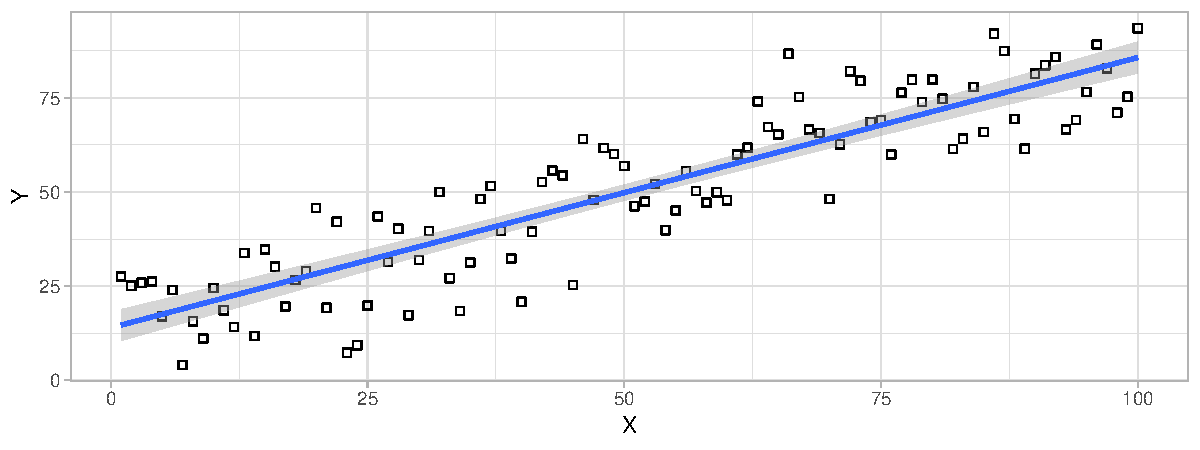
\includegraphics[width=\linewidth]{R/plots/linear_regression_SE}
        Linear regression line with 95\% confidence interval for $\hat{\beta}_0$, $\hat{\beta}_1$
    \end{figure}

\end{frame}

\begin{frame}[fragile]{Linear Regression in R}

    \begin{columns}
    \begin{column}{0.5\textwidth}
        Try the following code:
        {\tiny\begin{verbatim}
        # Define X and Y
        X <- rnorm(500, mean = 20, sd = 3)
        Y <- -1.3 * X + 70 + rnorm(length(X),
                                   mean = 0,
                                   sd = 10)
        
        # Put X, Y in a data frame
        df <- tibble(X = X, Y = Y)
        
        # Plot the regression line using ggplot2
        ggplot(df, mapping = aes(x = X, y = Y)) +
            geom_smooth(method = 'lm', se = T) +
            geom_point()
            
        # Fit a linear model using lm()
        linmod <- lm(Y ~ X)    
        print(linmod)
        \end{verbatim}}
    \end{column}
    \begin{column}{0.5\textwidth}
        \begin{figure}
            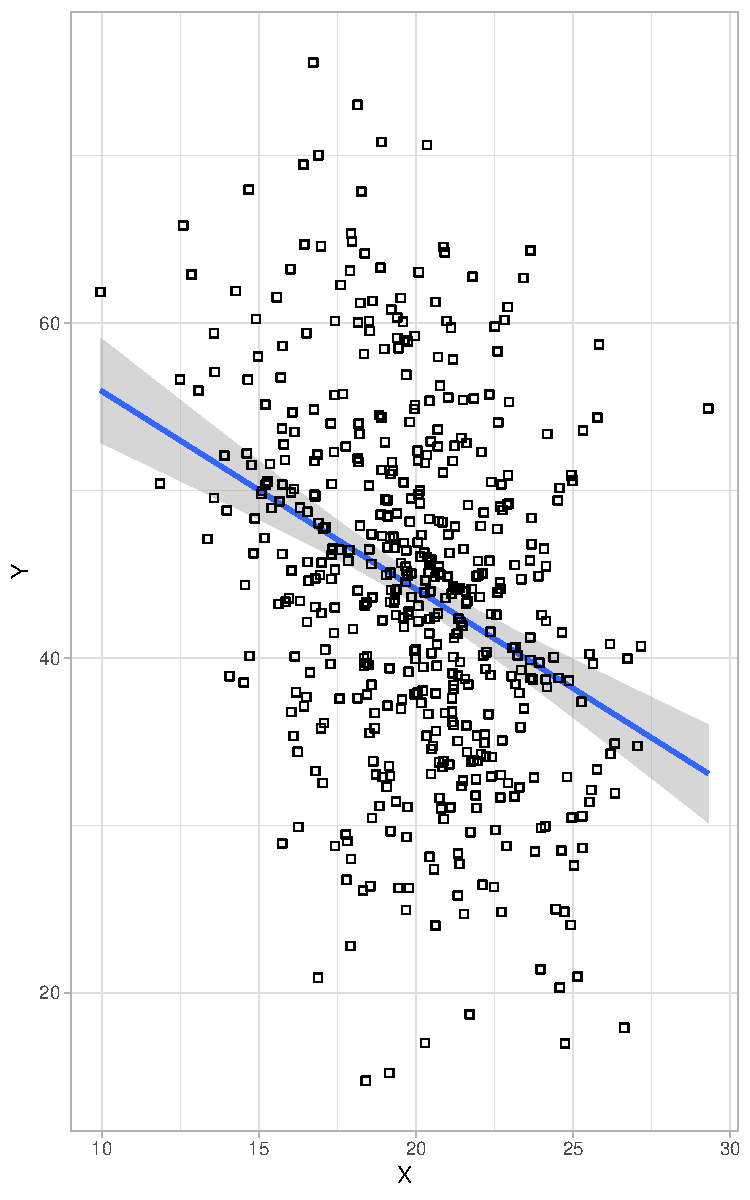
\includegraphics[width=0.8\linewidth]{R/plots/linear_regression_example}
        \end{figure}
    \end{column}
    \end{columns}

\end{frame}

\begin{frame}{Linear Regression in R}

    \begin{example}
        \medskip
        \begin{enumerate}
            \item Are the estimated coefficients close to the true coefficients?
            \item Plot the histogram of residuals for the previously fitted model. Is the distribution of residuals close to normal? Is the mean of residuals close to zero?
            \item What happens if you reduce/increase the noise in $Y$?
            \item Fit a linear model to a nonlinear relationship:\\
            {\small\texttt{X <- rnorm(500, mean = 1, sd = 3)}}\\
            {\small\texttt{Y <- X\^{}2 + rnorm(length(X), mean = 10, sd = 10)}}\\
            Is the distribution of residuals close to normal? Is the mean of residuals close to zero? Why?
        \end{enumerate}
    \end{example}

\end{frame}

\begin{frame}{Hypothesis Tests on the Coefficients}

    Standard errors of the coefficients can be used in hypothesis testing for relationships between variables. E.g.:
    \begin{itemize}
        \item $H_0$: There is no relationship between $X$ and $Y \Rightarrow \beta_1 = 0$
        \item $H_A$: There is some relationship between $X$ and $Y \Rightarrow \beta_1 \ne 0$
    \end{itemize}

    We need to determine whether $\hat{\beta}_1$ is sufficiently far from zero, taking into account the uncertainty $SE_{\hat{\beta}_1}$, before we can be confident that the real $\beta_1$ is non-zero.

\end{frame}

\begin{frame}{Hypothesis Tests on the Coefficients}

    First, we compute the $t$-statistic:
    \begin{equation*}
    t = \frac{\hat{\beta}_1 - 0}{SE_{\hat{\beta}_1}}
    \end{equation*}

    Afterwards, we compute the p-value and compare it with the assumed significance level $\alpha$ (e.g. 0.05). The p-value is computed based on the $t$-distribution with $df = n - v$ degrees of freedom, where $v$ is the number of model coefficients. $v = 2$ in the simple linear regression.
    
    If p-value~$< \alpha$, we reject the null hypothesis.
    
\end{frame}   
 
\begin{frame}[fragile]{Hypothesis Tests on the Coefficients}

    Analyze the following summary:

    {\tiny\begin{verbatim}
    > linmod <- lm(Y ~ X)
    > summary(linmod)
    
    Call:
    lm(formula = Y ~ X)
    
    Residuals:
    Min       1Q   Median       3Q      Max 
    -31.2473  -6.4663   0.0575   5.8874  27.5949 
    
    Coefficients:
                 Estimate    Std. Error  t value   Pr(>|t|)    
    (Intercept)  67.7640     3.0661      22.101    < 2e-16 ***
    X            -1.1834     0.1517      -7.802    3.6e-14 ***
    ---
    Signif. codes:  0 ‘***’ 0.001 ‘**’ 0.01 ‘*’ 0.05 ‘.’ 0.1 ‘ ’ 1
    
    Residual standard error: 10.04 on 498 degrees of freedom
    Multiple R-squared:  0.1089,	Adjusted R-squared:  0.1071 
    F-statistic: 60.88 on 1 and 498 DF,  p-value: 3.596e-14
    \end{verbatim}}

\end{frame}

\begin{frame}{Assessing the Accuracy of the Model}
    There are two main statistics used in assessing the accuracy of a linear model:
    \begin{itemize}
        \item RSE - absolute measure of error
        \item $R^2$ - relative measure of error
    \end{itemize}

    $R^2$ describes the proportion of variance explained. It always takes a value between 0 and 1.

    \begin{equation}
    R^2 = \frac{TSS - RSS}{TSS} = 1 - \frac{RSS}{TSS}
    \end{equation}
    
    where $TSS = \sum(y_i - \bar{y})^2$ is the \emph{total sum of squares}.

\end{frame}

\begin{frame}{TSS and RSS in R$^2$}
    \begin{equation*}
    R^2 = \frac{TSS - RSS}{TSS} = 1 - \frac{RSS}{TSS}
    \end{equation*}

    \begin{description}
        \item[TSS] corresponds to the amount of variability inherent in the response before the regression is performed
        \item[RSS] corresponds to the amount of variability that is left unexplained after performing the regression
    \end{description}

    In example, if $Y = f(X) = \beta_0 + \beta_1 X$ and $R^2 = 0.72$,\\ then \emph{72\% of variability in $Y$ can be explained using $X$}.
\end{frame}

\begin{frame}{Binary Classification: Precision and Recall}
    \begin{columns}
        \begin{column}{0.6\linewidth}
            If a model is used for binary classification (True/False), it's accuracy can be characterized with \emph{precision} and \emph{recall}.
            
            ``False positive" is often called ``Type I error". ``False negative" is often called ``Type II error".
            
            \vspace{40pt}
            {\tiny
            Image:
            \vspace{8pt}
            
            Walber (CC BY-SA 4.0)
            
            https://creativecommons.org/licenses/by-sa/4.0
            
            https://commons.wikimedia.org/wiki/File:Precisionrecall.svg}
        \end{column}
        \begin{column}{0.4\linewidth}
            \vspace{10pt}
            
            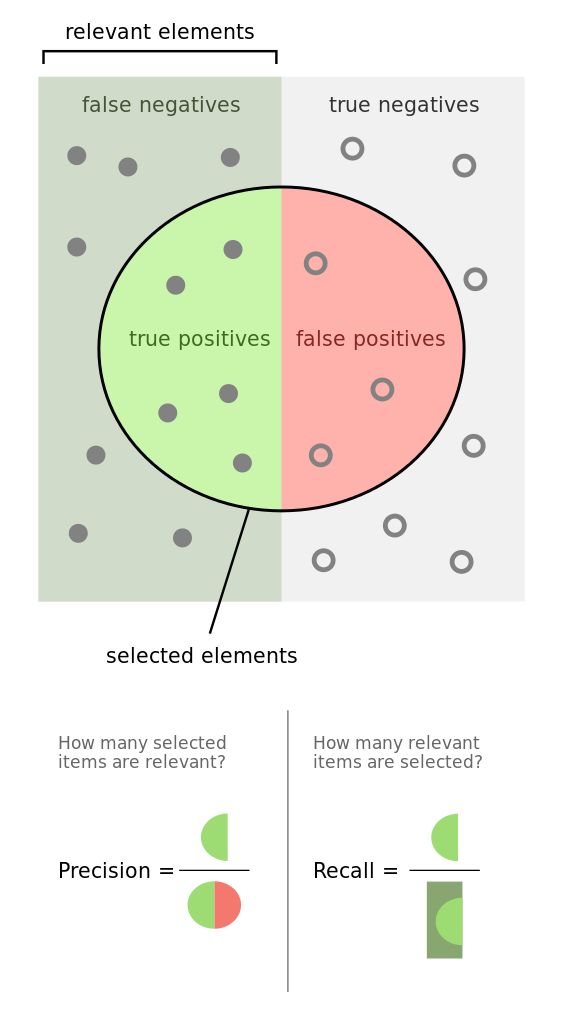
\includegraphics[width=0.95\linewidth]{gfx/precisionrecall}
        \end{column}
    \end{columns}
\end{frame}

\begin{frame}[fragile]{Multiple Linear Regression}
    It is possible to include multiple predictors in the linear regression:
    
    \begin{equation*}
    Y = \beta_0 + \beta_1 X_1 + \beta_2 X_2 + ... + \beta_n X_n + \epsilon
    \end{equation*}

    In R:
    \begin{verbatim}
    m <- lm(Y ~ X1 + X2 + X3)
    \end{verbatim}
\end{frame}

\begin{frame}{Multiple Linear Regression: Example With 2 Predictors}
    \begin{columns}
        \begin{column}{0.5\linewidth}
            \begin{figure}
            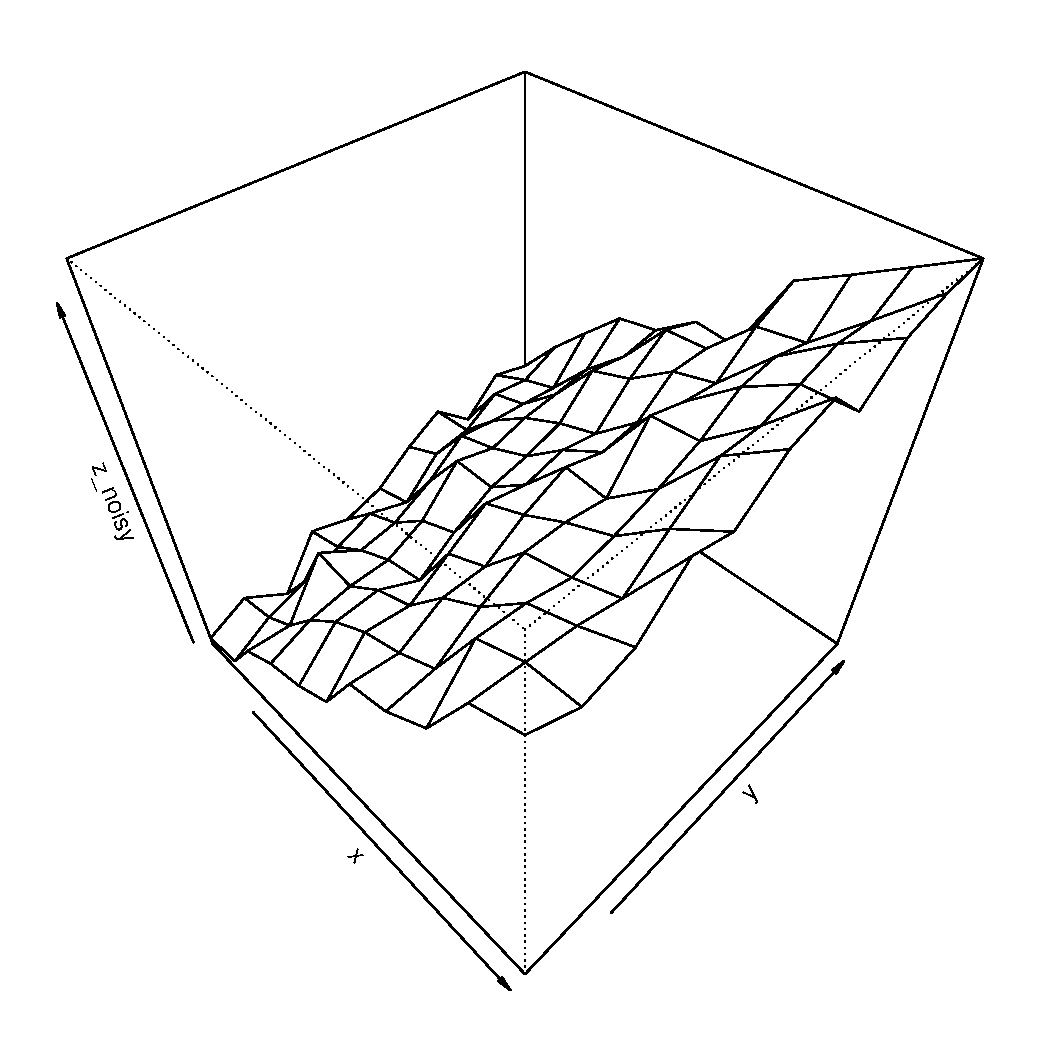
\includegraphics[width=\linewidth]{R/plots/regression-2d-noisy}
            Actual data
            \end{figure}
        \end{column}
        \begin{column}{0.5\linewidth}
            \begin{figure}
            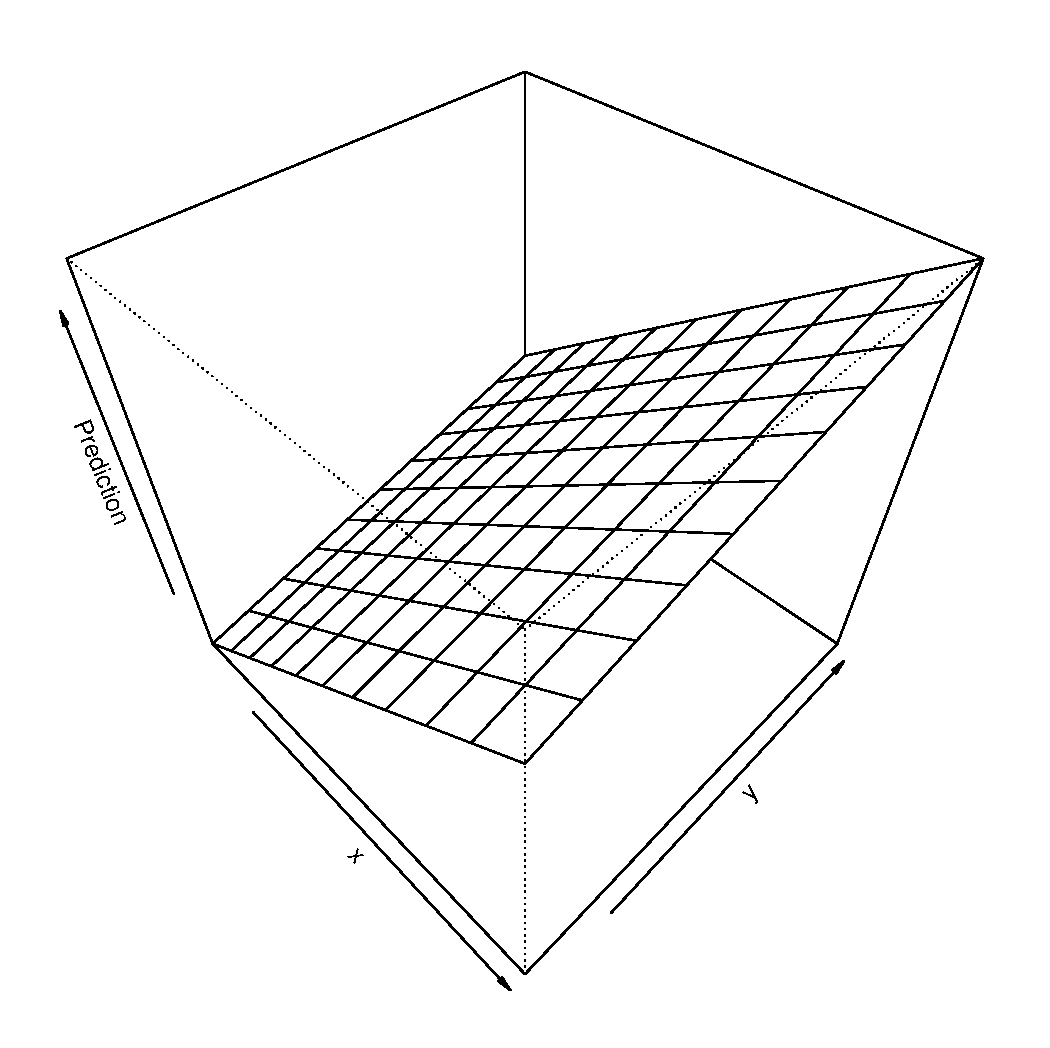
\includegraphics[width=\linewidth]{R/plots/regression-2d-clean}
            Fitted linear model
            \end{figure}
        \end{column}
    \end{columns}
\end{frame}

\begin{frame}{F-statistic}
    In addition to the p-values calculated for each predictor,
    the {\small \texttt{lm()}} function calculates a so-called the F-statistic.
    The F-statistic is used to test the following hypothesis:
    \begin{align*}
        H_0&: \beta_1 = \beta_2 = ... = \beta_p = 0 \\
        H_a&: \text{at least on $\beta_j$ is non-zero}\\
    \end{align*}
    F-statistic is calculated based on the F-distribution, which is most notably
    used in the analysis of variance (ANOVA - to be introduced later).

    If the p-value associated with the F-statistic is close to zero, we have
    a strong evidence that at least one coefficient is non-zero. This insight
    is especially useful if there are many (hundreds or thousands) coefficients.
\end{frame}

\begin{frame}{F-statistic}
    E.g. if there are 100 predictors and $H_0: \beta_1 = \beta_2 = ... = \beta_{100} = 0$ is true,
    then about 5\% of the p-values will be below 0.05 simply by chance!

    \emph{The F-statistic doesn't suffer from this problem.}
\end{frame}

\begin{frame}{Predictor Selection}
    Most often the response variable is dependent on a subset of predictors.

    To find the appropriate predictors:
    \begin{enumerate}
        \item Examine the F-statistic and the associated p-value
        \item Use expert knowledge
        \item Test different models and compare $R^2$ (manual testing feasible only for small number of predictors)
    \end{enumerate}

    Testing of different model configurations can be automated using:
    \begin{itemize}
        \item Forward selection (start with none, add 1-by-1)
        \item Backward selection (start with all, remove 1-by-1)
        \item Mixed selection (start with none, add 1-by-1, remove if p-value grows too much)
    \end{itemize}
\end{frame}

\begin{frame}[fragile]{Making Predictions}
    Once the model coefficients are estimated, it is straightforward to use the model.
    In R the function for feeding new data to a model is called {\small\texttt{predict.lm()}}
    (see also {\small\texttt{predict()}}).

    \begin{verbatim}
        # Training
        X1 <- rnorm(10)
        X2 <- rnorm(10)
        Y <- 2 * X1 - 0.7 * X2
        m <- lm(Y ~ X1 + X2)

        # Prediction
        df <- data.frame(X1 = 1, X2 = 1)
        Y_predict <- predict(m, df)  # Returns 1.3
    \end{verbatim}
\end{frame}

\begin{frame}{Polynomial Regression}
    Polynomial regression is a special form of regression analysis in which the relationship
    between the outcome and predictor variables is modelled using a polynomial, e.g.:
    \begin{equation*}
        Y = \beta_0 + \beta_1 X_1 + \beta_2 X_1^2 + \beta_3 X_1 X_2
    \end{equation*}

    Even though the polynomial regression fits a non-linear function to data,
    the coefficients are estimated in the same way as in the multiple linear
    regression, because the regression function is linear with respect to the
    parameters $\beta_j$.
\end{frame}

\begin{frame}[fragile]{Polynomial Regression}
    \begin{columns}
        \begin{column}{0.5\linewidth}
            In example, to find the coefficients for the following model:
            \begin{equation*}
                Y = \beta_0 + \beta_1 X_1^3
            \end{equation*}
            use the following command in R:
            \begin{verbatim}
      lm(Y ~ I(X1^3))
            \end{verbatim}
            {\small\texttt{I()}} has to be used, because {\small\texttt{\^}}
            has a special meaning in formulas. Type {\small\texttt{?formula}}
            for more info.
        \end{column}
        \begin{column}{0.5\linewidth}
            \begin{figure}
                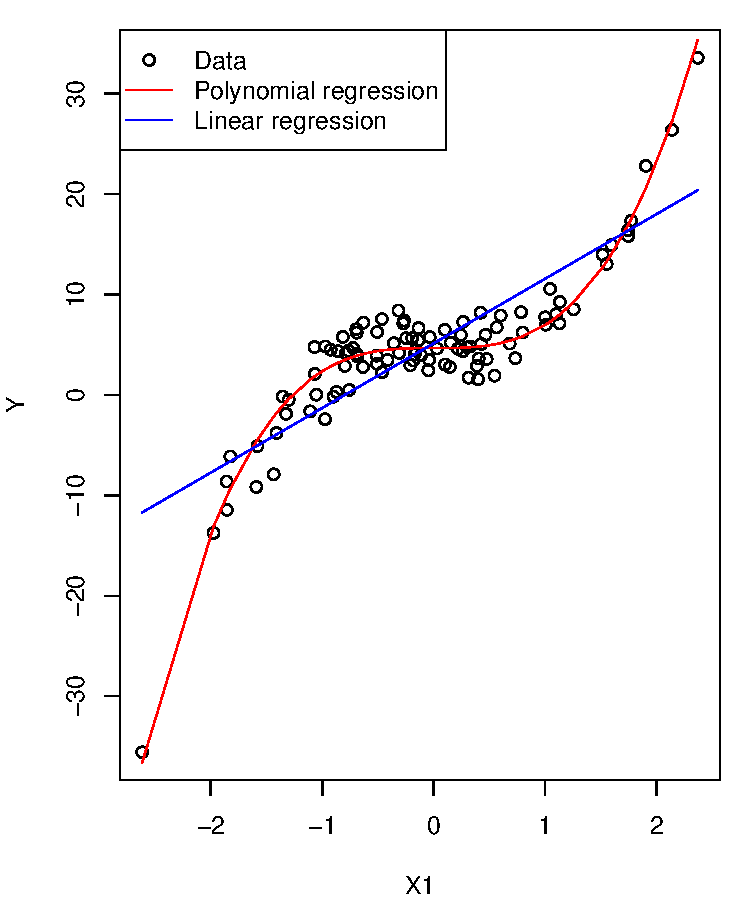
\includegraphics[width=\linewidth]{R/plots/poly_regression}
            \end{figure}
        \end{column}
    \end{columns}
\end{frame}

\begin{frame}{Formulas in Polynomial Regression}
    R formulas might seem peculiar at first, but they are actually very handy,
    especially in the cases with many predictor variables:
    \vspace*{1cm}

    \begin{tabular}{l l}
        Function & Regression formula \\ \hline
        $Y = \beta_0 + \beta_1 X_1 + \beta_2 X_1^2$ & lm(Y $\sim$ X1 + I(X $\hat{}$ 2))\\
        $Y = \beta_0 + \beta_1 X_1 X_2$ & lm(Y $\sim$ X1:X2) \\
        $Y = \beta_0 + \beta_1 X_1 + \beta_2 X_2 + \beta_3 X_1 X_2$ & lm(Y $\sim$ X1*X2) \\
        $Y = \beta_1 X^3$ & lm(Y $\sim$ I(X $\hat{}$ 3) - 1) \\
        $Y = \beta_0 + \sum_i \beta_i X_i$ & lm(Y $\sim$ ., data = df)
    \end{tabular}
\end{frame}

\begin{frame}{Energy Efficiency Data Set}
    \begin{example}
        \begin{itemize}
            \item Download the following data set:\\
            {\small \url{http://archive.ics.uci.edu/ml/datasets/Energy+efficiency}}
            \item Choose predictor variables and fit a linear model. Try to minimize $R^2$.
            \item Plot model predictions vs. validation data.
            \item Optional: divide the data set into training (80\%) and validation subsets (20\%) (random sample!).
        \end{itemize}

        {\small \textbf{Related paper:} A. Tsanas, A. Xifara: `Accurate quantitative estimation of energy performance of residential buildings using statistical machine learning tools', Energy and Buildings, Vol. 49, pp. 560-567, 2012}
    \end{example}
\end{frame}

\begin{frame}{Energy Efficiency Data Set}
Variables:
\begin{description}
    \item[X1] Relative compactness 
    \item[X2] Surface area
    \item[X3] Wall area
    \item[X4] Roof area
    \item[X5] Overall height
    \item[X6] Orientation
    \item[X7] Glazing area
    \item[X8] Glazing area distribution
    \item[Y1] Heating load
    \item[Y2] Cooling load
\end{description}
\end{frame}

\begin{frame}{Energy Efficiency Data Set}
    \begin{figure}
    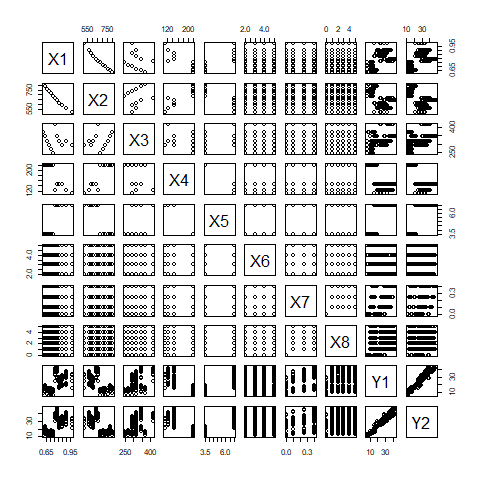
\includegraphics[width=0.75\linewidth]{R/plots/energy-efficiency-df}
    \end{figure}
\end{frame}

\begin{frame}{Energy Efficiency Data Set}
    \begin{figure}
        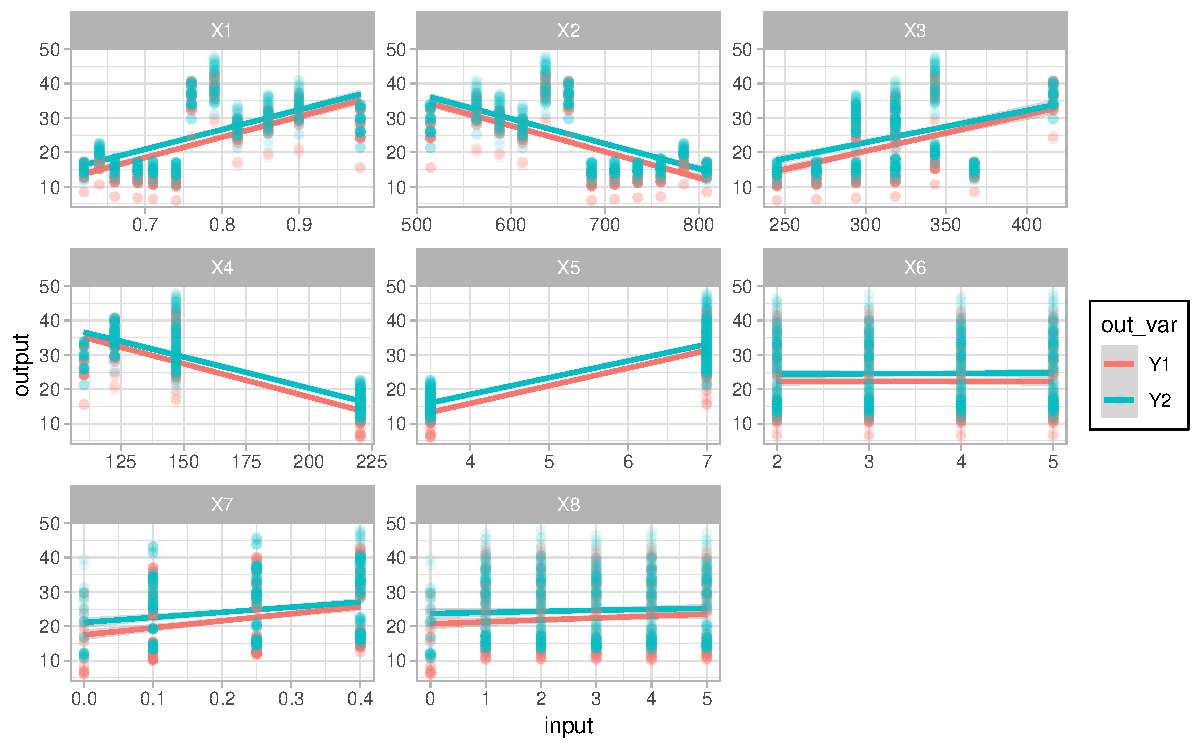
\includegraphics[width=\linewidth]{R/plots/energy-efficiency-ggplot}
        Simple linear regression is insufficient. Can you get better results with multiple regression?
    \end{figure}
\end{frame}
